\chapter{Arquitectura del sistema}
\label{ch:arquitectura}

\section{Diagrama de paquetes}

\subsection{API}

El diagrama de paquetes de la \acrshort{api} es la \fref{fig:diagrama_paquetes_api}. Esta \acrshort{api} se cimentará sobre el \textbf{Server}, que será el punto de inicio del sistema. Esta entidad iniciará los funciones de sus tres componentes principales: \textbf{App}, con la \acrshort{api} \acrshort{rest} desarrollada en Express (\fref{lib:api:express}); \textbf{Mongo}, con el cliente Mongoose (\fref{lib:api:mongoose}) de la base de datos; y \textbf{socketio} (\fref{lib:api:socket_io}), con la lógica de la \acrshort{api} WebSocket. 

Todo el funcionamiento de la \acrshort{api} \acrshort{rest} se haya en el paquete \textbf{routers}, el cuál está dividido a su vez en paquetes relativos a los \glspl{endpoint} ofrecidos, paquetes que contienen sus enrutadores respectivos. Por otro lado, el funcionamiento de la \acrshort{api} WebSocket está en el paquete \textbf{sockets} y tiene una distribución similar pero con manejadores de eventos en vez de enrutadores.

\begin{figure}[H]
    \centering
    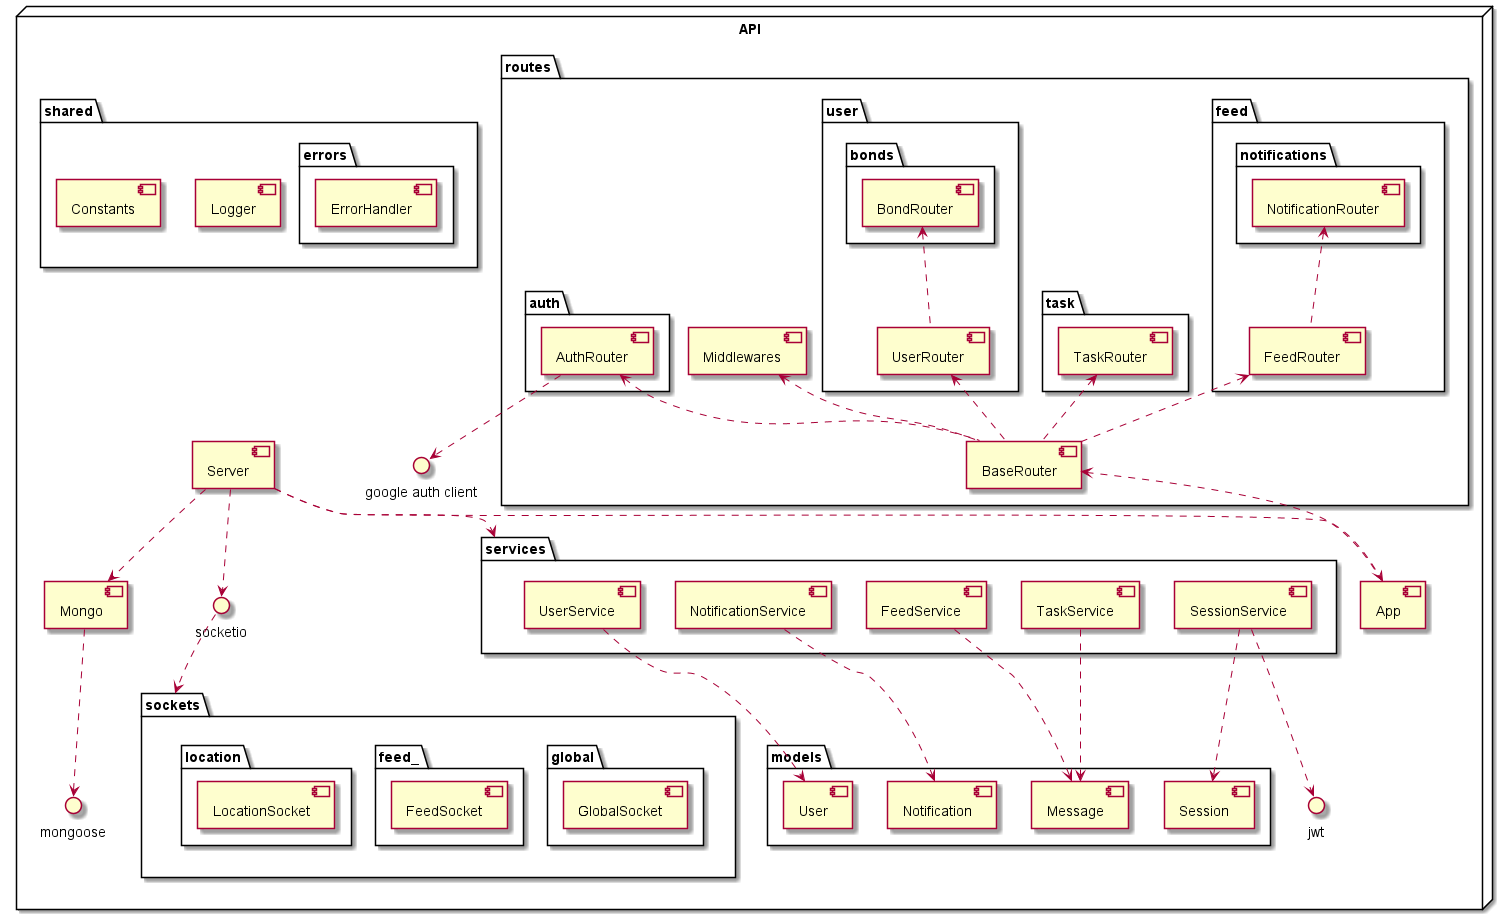
\includegraphics[width=1\textwidth]{images/Diseño/DiagramaPaquetesApi.png}
    \caption{Diagrama de paquetes de la API}
    \label{fig:diagrama_paquetes_api}
\end{figure}

Los paquetes \textbf{services} y \textbf{models} contienen toda la lógica de datos del sistema y son accedidos por las entidades de los dos paquetes mencionados con anterioridad. Las entidades del modelo de datos (ver \fref{ch:modelo_datos}) están en el paquete \textbf{models} mientras que los servicios que gestionan la persistencia y recuperación de dichas entidades están en \textbf{services}. Por último, en el paquete \textbf{shared} se encuentran funciones, datos y entidades comunes a todos los componentes del sistema como los errores, las cadenas de texto o el registro del sistema.

\subsection{Aplicación móvil}

Como se puede ver en la \fref{fig:diagrama_paquetes_app}, la aplicación móvil tiene un diagrama de paquetes que sigue la arquitectura de capas del \acrlong{mvvm} que ya planteamos en la fase de análisis en la \fref{sec:subsistema_app}. La parte clave es el paquete de \textbf{ui}, que se encuentra dividido a su vez en paquetes relativos a las distintas pantallas que tendrá la aplicación móvil, conteniendo la actividad, el modelo de la vista y cualquier otra pantalla, diálogo o fragmento auxiliar de la misma.

La interfaz de usuario se comunicará con los los repositorios del paquete \textbf{repositories} por medio de los objetos de valor (o \emph{value objects}) que se definirán en el paquete \textbf{vo}. Por último, la capa más profunda de la aplicación es aquella que se conectará con las \acrshort{api}, lo que da nombre al paquete en el que se albergan \textbf{api}. Este paquete expondrá una interfaz para el manejo del WebSocket y una factoría para los servicios del paquete \textbf{services}.

\begin{figure}[H]
    \centering
    \makebox[\textwidth][c]{
        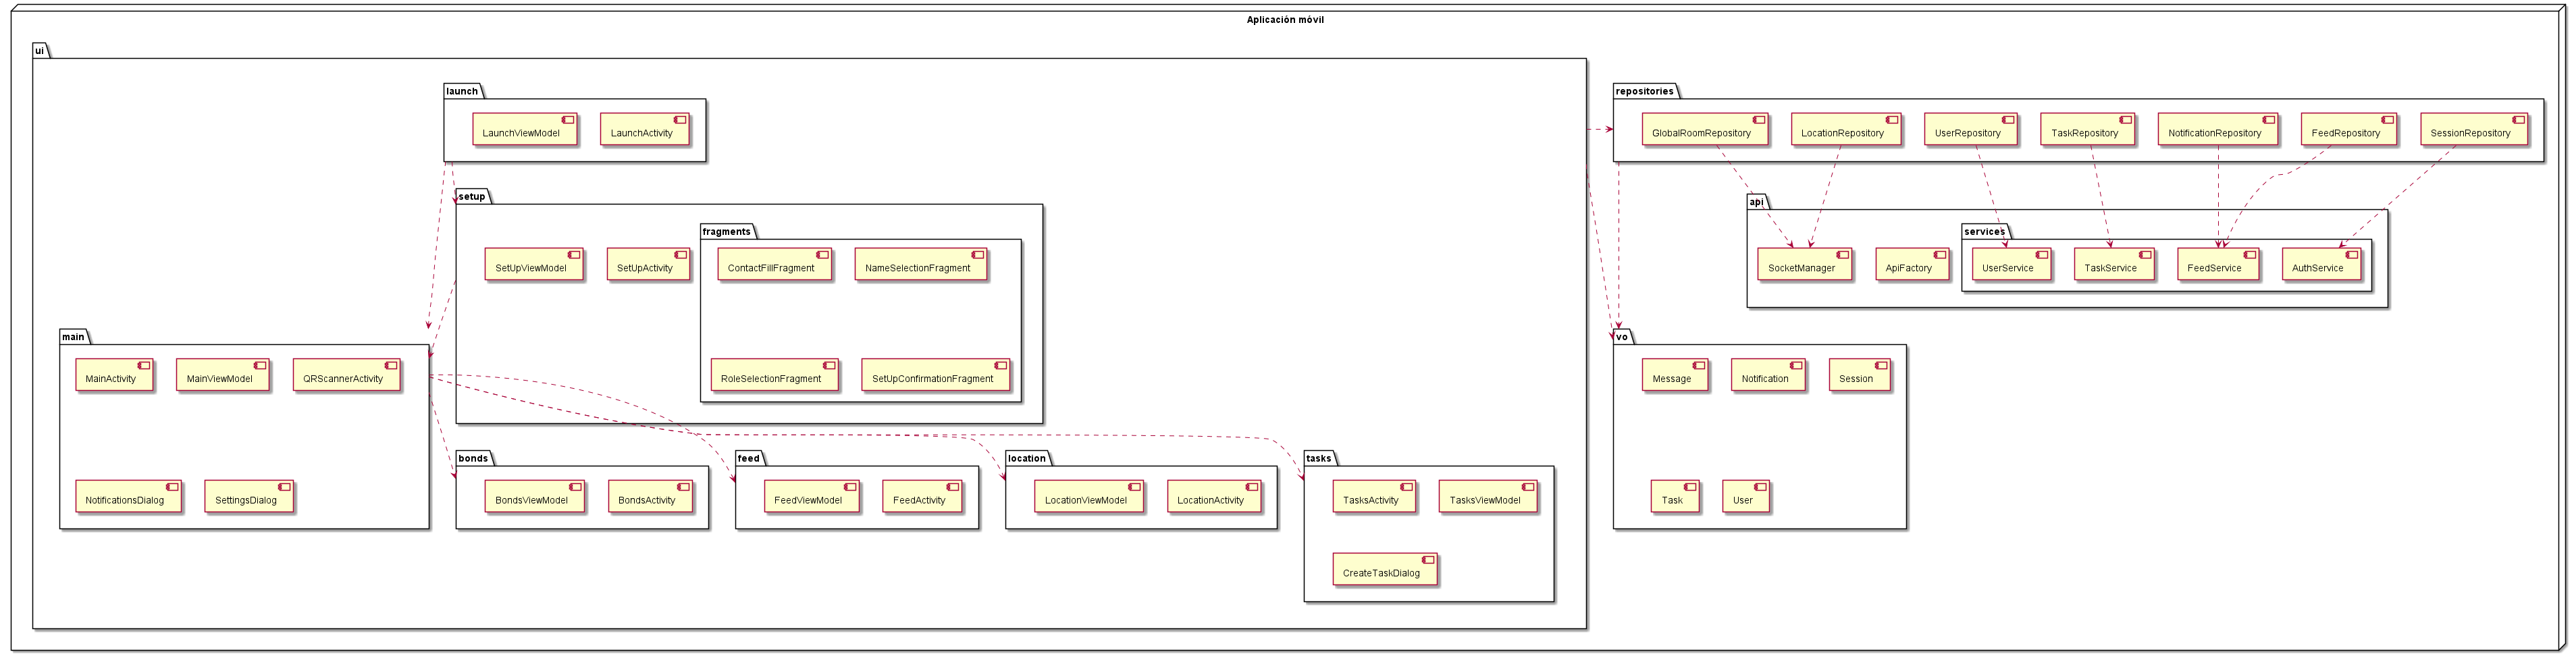
\includegraphics[width=1.1\textwidth]{images/Diseño/DiagramaPaquetesApp.png}
    }
    \caption{Diagrama de paquetes de la aplicación móvil}
    \label{fig:diagrama_paquetes_app}
\end{figure}

\section{Diagrama de despliegue}

La aplicación móvil se instalará en los dispositivos Android de los usuarios por medio de la \acrshort{apk} o el \acrlong{aab} de la aplicación. La \acrshort{api} se desplegará en una instancia AppService de Microsoft Azure como la que se especificó en el \fref{sec:despliegue_api}. La base de datos estará hospedada en el servicio en la nube de MongoDB, MongoDB Atlas. Las aplicaciones de los clientes se comunicarán con la \acrshort{api} por medio de peticiones \acrshort{http} \acrshort{rest} o de eventos a través del WebSocket. La \acrshort{api}, por su parte, se comunicará por red con la base de datos. Esto todo puede visualizarse en la \fref{fig:diagrama_despliegue}.

\begin{figure}[H]
    \centering
    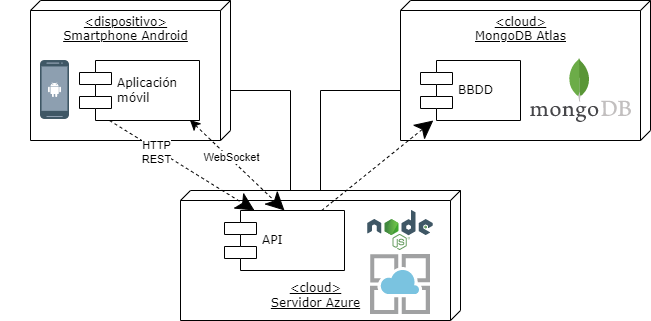
\includegraphics[width=0.65\textwidth]{images/Diseño/DiagramaDespliegue.drawio.png}
    \caption{Diagrama de despliegue del sistema}
    \label{fig:diagrama_despliegue}
\end{figure}

\begin{figure}[H]
    \centering
    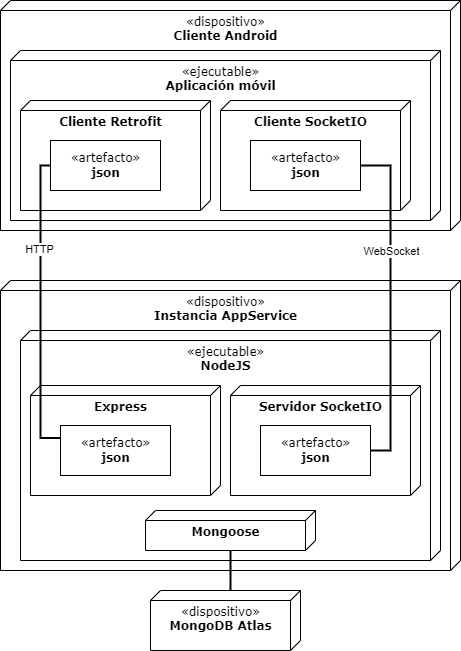
\includegraphics[width=0.6\textwidth]{images/Diseño/DiagramaComponentes.drawio.png}
    \caption{Diagrama de componentes del sistema}
    \label{fig:diagrama_componentes}
\end{figure}

\section{Diagrama de componentes}

El sistema estará compuesto por tres componentes principales análogos a las entidades de la sección anterior. Por un lado estará el \textbf{cliente}, que será el dispositivo del usuario y sobre el que se ejecutará la aplicación móvil; por otro lado estará la \textbf{API} ejecutada sobre una instancia de AppService; y por último, la \textbf{base de datos} alojada en MongoDB Atlas. En la aplicación habrá un cliente \acrshort{http} y otro cliente Socket.io (\fref{lib:api:socket_io}) que se comunicarán con los componentes Express (\fref{lib:api:express}) y servidor Socket.io de la \acrshort{api}, respectivamente. La comunicación definitiva entre la \acrshort{api} y la base de datos se llevará a cabo con el componente Mongoose (\fref{lib:api:mongoose}). Véase \fref{fig:diagrama_componentes}.
